\PassOptionsToPackage{naturalnames}{hyperref}
\RequirePackage{luatex85}
\documentclass{article}
\usepackage{geometry}
%\usepackage{fullpage}
\usepackage{parskip}
\usepackage{physics}
\usepackage{amsmath}
\usepackage{amssymb}
\usepackage{xcolor}
\usepackage[colorlinks,linkcolor=blue,citecolor=green]{hyperref}
\usepackage{array}
\usepackage{longtable}
\usepackage{multirow}
\usepackage{comment}
\usepackage{graphicx}
\usepackage{cite}
\usepackage{amsfonts}
\usepackage{bm}
\usepackage{slashed}
\usepackage{dsfont}
\usepackage{mathtools}
\usepackage[compat=1.1.0]{tikz-feynman}
\usepackage{simplewick}
%\usepackage{fourier}
%\usepackage{slashbox}
%\usepackage{intent}
\usepackage{mathrsfs}
\usepackage{xparse}
\usepackage{enumerate}
%\usepackage{axodraw4j}
\usepackage[toc,page]{appendix}
\usepackage{multicol}

%\usepackage{luatexja-fontspec}

\geometry{left=0.5cm,right=0.5cm,top=1.5cm,bottom=2cm}

\newcommand{\gm}{\gamma^{\mu}}
\newcommand{\gn}{\gamma^{\nu}}
\newcommand{\gs}{\gamma^{\sigma}}
\newcommand{\gr}{\gamma^{\rho}}
\newcommand{\gnr}{g^{\nu\rho}}
\newcommand{\gmr}{g^{\mu\rho}}
\newcommand{\gms}{g^{\mu\sigma}}
\newcommand{\gns}{g^{\nu\sigma}}
\newcommand{\vbp}{\vb{p}}
\newcommand{\vbk}{\vb{k}}
\newcommand{\g}{\gamma}
\renewcommand{\a}{\alpha}
\renewcommand{\b}{\beta}
\renewcommand{\t}{\theta}
\newcommand{\la}{\lambda}
\newcommand{\p}{\phi}
\newcommand{\vp}{\varphi}
\newcommand{\s}{\sigma}
\newcommand{\G}{\Gamma}
\newcommand{\pars}{\slashed\partial}
\newcommand{\ps}{\slashed p}
\newcommand{\ks}{\slashed k}
\newcommand{\lag}{\mathcal{L}}
\newcommand{\da}{^{\dagger}}
\newcommand{\sm}{^{\mu}}
\newcommand{\sn}{^{\nu}}
\newcommand{\smn}{^{\mu\nu}}
\newcommand{\Dm}{D^{\mu}}
\newcommand{\dm}{\partial^{\mu}}
\newcommand{\Asquare}{A^{\mu}A_{\mu}}
\newcommand{\partialsquare}[2]{\partial^{\mu}{#1}\partial_{\mu}{#2}}

%\setmainjfont[BoldFont=FandolSong-Bold]{FandolSong-Regular}
%\setsansjfont{FandolSong-Bold}
%\setlength{\parindent}{2em}
%\linespread{1.2}

\title{Scalar QED}
\author{Yingsheng Huang}
\begin{document}
\maketitle
\section{Hydrogen Wavefunction Divergence in Klein-Gordon Equation and Schr\"odinger Equation}


\section{Non-relativistic Scalar QED (NRSQED) Matching}
\subsection{Feynman Rules}
\subsubsection{Scalar QED (SQED)}
Lagrangian
\begin{align}
  \lag_{SQED}=\abs{D_{\mu}\phi}^2-m^2\abs{\phi}^2+\Phi_v^*iv\cdot D\Phi_v
  \label{SQEDLAG}
\end{align}
with
\begin{align*}
  D_{\mu}\phi=\partial_{\mu}\phi+ieA_{\mu}\phi
\end{align*}
and 
\begin{align*}
  D_{\mu}\Phi_v=\partial_{\mu}\Phi-iZeA_{\mu}\Phi_v
\end{align*}
But note that no $\vb{A}$ can appear in actual calculation because here only static scalar potential exists. 
And the Feynman rules
\begin{multicols}{2}
  \begin{align*}
	\feynmandiagram[small,horizontal=a to b]{
	a -- [momentum=$p$] b,
    };&=\frac{i}{p^2-m^2+i\epsilon}\\
	\feynmandiagram[small,horizontal=a to o,baseline=(o.base)]{
	  a -- [momentum=$p_1$] o,
	  o -- [momentum=$p_2$] b,
	  c -- [photon] o,
	};&=-ie(p_1^{\mu}+p_2^{\mu})\\
	\feynmandiagram[small,horizontal=a to b,baseline=(o.base)]{
	  a -- [momentum'=$p_1$] o -- [momentum'=$p_2$] b,
	  c -- [photon] o,
	  d -- [photon] o,
	};&=2ie^2g^{\mu\nu}
  \end{align*}
  \begin{align*}
	\feynmandiagram[small,horizontal=a to b]{
		a -- [momentum=$mv+k$,double distance=1pt] b,
	};&=\frac{i}{v\cdot k}\\
	\feynmandiagram[small,baseline=(o.base)]{
	  a -- [double distance=1pt] o -- [double distance=1pt] b,
	  c -- [photon] o,
	};&=iZev^{\mu}\\\\\\
	\feynmandiagram[small,horizontal=a to b]{
	  a [particle=$A^0$] -- [photon,momentum=$q$] b,
	};&=\frac{i}{\vb{q}^2}
  \end{align*}
\end{multicols}
\subsubsection{NRSQED}
Lagrangian
\begin{align}
  \lag_{NRSQED}=\varphi^*\pqty{iD_0+\frac{\vb{D}^2}{2m}}\varphi+\delta\lag +\Phi_v^*iv\cdot D\Phi_v
  \label{NRSQEDLAG}
\end{align}
with the same notation above. Here $\vb{D}=\nabla-ie\vb{A}$.

Feynman rules are also the same except for the scalar electron side which becomes
\begin{align*}
	\feynmandiagram[small,horizontal=a to b]{
	a -- [momentum=$p$] b,
    };=\frac{i}{E-\frac{\vb{p}^2}{2m}+i\epsilon}\;\;\;\;\;\;\;\;\;\;\;\;\;\;\;
	\feynmandiagram[small,horizontal=a to o,baseline=(o.base)]{
	  a -- [momentum=$p_1$] o,
	  o -- [momentum=$p_2$] b,
	  c [particle=$A^0$] -- [photon] o,
	};=-ie
\end{align*}
We can ignore all interacting terms involving $\vb{A}$. 

Since we need to match it to $\mathcal{O}(v^2)$ order
\begin{align}
  \delta\lag=(D_0\varphi)^*(D_0\varphi)=\frac{\dot{\varphi}^*\dot{\varphi}}{2m}+\frac{e^2\varphi^*\varphi A_0^2}{2m}-\frac{ie}{2m}A_0(\varphi^*\dot{\varphi}-\dot{\varphi}^*\varphi)
  \label{deltaLAG}
\end{align}
and it changes the Feynman rules to\footnote{In this note, $p^0$ is the zero component of relativistic four momentum, and $E=p^0-m$. }
\begin{align*}
	\feynmandiagram[small,horizontal=a to o,baseline=(o.base)]{
	  a -- [momentum=$p_1$] o,
	  o -- [momentum=$p_2$] b,
	  c [particle=$A^0$] -- [photon] o,
	};=-ie(1+\frac{E_1+E_2}{2m})\;\;\;\;\;
	\feynmandiagram[small,horizontal=a to b,baseline=(o.base)]{
	  a -- [momentum'=$p_1$] o -- [momentum'=$p_2$] b,
	  c [particle=$A^0$] -- [photon] o,
	  d [particle=$A^0$] -- [photon] o,
	};&=\frac{ie^2}{2m}
\end{align*}<++>

Since we rescaled $\phi$ by $\frac{1}{\sqrt{2m}}$ to get $\varphi$, the in/out states are also changed. We must multiply them by $\sqrt{2m}$ to compensate that change. 
\subsection{LO}
\subsubsection{SQED}
\begin{align*}
  i\mathcal{M}_{SQED}^{(0)}&=\feynmandiagram[horizontal=i1 to f1,layered layout,inline=($(a)!0.5!(c)$),medium]{
	i1[particle=$P_N$] -- [double distance=1pt] a -- [double distance=1pt] f1[particle=$P_N$],
	i2[particle=$p_1$] -- [] c -- [] f2[particle=$p_2$],
	{ [same layer] a -- [photon,momentum'=$q$] c},
  };=-e^2v^{0}\frac{i(p_1^0+p_2^0)}{\vb{q}^2}=-e^2v^0\frac{i}{\vb{q}^2}(2m+E_1+E_2)
\end{align*}
\subsubsection{NRSQED}
 \begin{align*}
   i\mathcal{M}_{NRSQED}^{(0)}&=\feynmandiagram[horizontal=i1 to f1,layered layout,inline=($(a)!0.5!(c)$),medium]{
	i1[particle=$P_N$] -- [double distance=1pt] a -- [double distance=1pt] f1[particle=$P_N$],
	i2[particle=$p_1$] -- [] c -- [] f2[particle=$p_2$],
	{ [same layer] a -- [photon,momentum'=$q$] c},
  };=-2me^2v^{0}\frac{i(1+\frac{E_1+E_2}{2m})}{\vb{q}^2}
\end{align*}
\subsection{NLO}
\subsubsection{SQED}
\begin{align*}
  i\mathcal{M}_{SQED}^{(1)}&=\feynmandiagram[horizontal=i1 to f1,layered layout,inline=($(a)!0.5!(c)$),medium]{
	i1[particle=$P_N$] -- [double distance=1pt] a -- [double distance=1pt,momentum=$P_N-k^0$] b -- [double distance=1pt] f1[particle=$P_N$],
	i2[particle=$p_1$] -- [] c -- [momentum=$p_1+k$] d -- [] f2[particle=$p_2$],
	{ [same layer] a -- [photon,momentum'=$k$] c},
	{ [same layer] b -- [photon,rmomentum=$k-q$] d},
  };
  +
  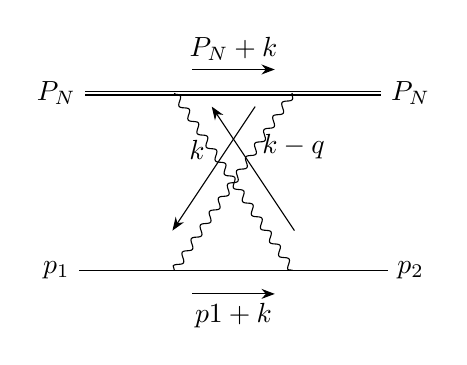
\begin{tikzpicture}[baseline=($(a)!0.5!(c)$)]
	\begin{feynman}
	  \diagram[horizontal=i1 to f1,layered layout,medium]{
		i1[particle=$P_N$] -- [double distance=1pt] a -- [double distance=1pt,momentum=$P_N+k$] b -- [double distance=1pt] f1[particle=$P_N$],
	i2[particle=$p_1$] -- [] c -- [momentum'=$p1+k$] d -- [] f2[particle=$p_2$],
	{ [same layer] a --[draw=none] c},
	{ [same layer] b-- [draw=none] d},
  };
	  \diagram*{
		(a) -- [photon,rmomentum=$k-q$] (d),
		(b) -- [photon,momentum'=$k$] (c),
	  };
	\end{feynman}
  \end{tikzpicture}
  +
  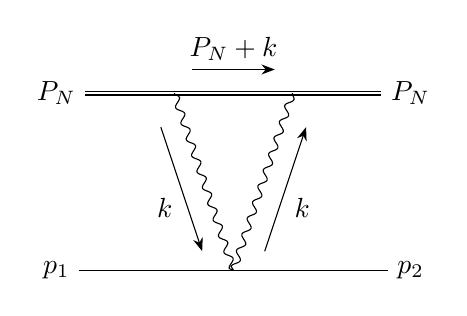
\begin{tikzpicture}[baseline=($(a)!0.5!(c)$)]
	\begin{feynman}
	  \diagram[horizontal=i1 to f1,layered layout,medium]{
		i1[particle=$P_N$] -- [double distance=1pt] a -- [double distance=1pt,momentum=$P_N+k$] b -- [double distance=1pt] f1[particle=$P_N$],
		i2[particle=$p_1$] -- [] c -- [] d -- [] f2[particle=$p_2$],
		{ [same layer] a --[draw=none] c},
		{ [same layer] b-- [draw=none] d},
	  };
	  \vertex at ($(c)!0.5!(d)$) (f);
	  \diagram*{
		(a) -- [photon,momentum'=$k$] (f),
		(b) -- [photon,rmomentum=$k$] (f),
	  };
	\end{feynman}
  \end{tikzpicture}
\end{align*}
\begin{align*}
  \feynmandiagram[horizontal=i1 to f1,layered layout,inline=($(a)!0.5!(c)$),medium]{
	i1[particle=$P_N$] -- [double distance=1pt] a -- [double distance=1pt,momentum=$P_N-k^0$] b -- [double distance=1pt] f1[particle=$P_N$],
	i2[particle=$p_1$] -- [] c -- [momentum=$p_1+k$] d -- [] f2[particle=$p_2$],
	{ [same layer] a -- [photon,momentum'=$k$] c},
	{ [same layer] b -- [photon,rmomentum=$k-q$] d},
  };=-e^2v^{0}\int\frac{\dd^4k}{(2\pi)^4}\frac{i}{\vb{k}^2}\frac{}{}<+content+>
\end{align*}<++>
\begin{align*}
  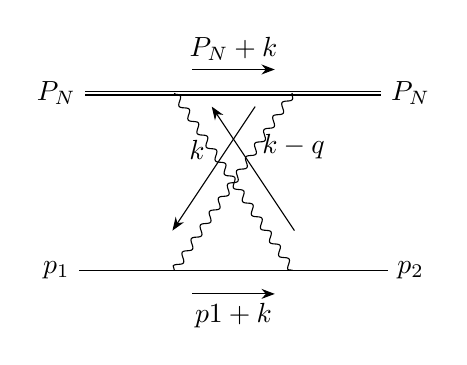
\begin{tikzpicture}[baseline=($(a)!0.5!(c)$)]
	\begin{feynman}
	  \diagram[horizontal=i1 to f1,layered layout,medium]{
		i1[particle=$P_N$] -- [double distance=1pt] a -- [double distance=1pt,momentum=$P_N+k$] b -- [double distance=1pt] f1[particle=$P_N$],
	i2[particle=$p_1$] -- [] c -- [momentum'=$p1+k$] d -- [] f2[particle=$p_2$],
	{ [same layer] a --[draw=none] c},
	{ [same layer] b-- [draw=none] d},
  };
	  \diagram*{
		(a) -- [photon,rmomentum=$k-q$] (d),
		(b) -- [photon,momentum'=$k$] (c),
	  };
	\end{feynman}
  \end{tikzpicture} <+content+>
\end{align*}<++>
\begin{align*}
  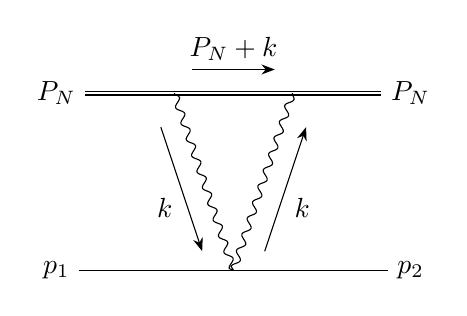
\begin{tikzpicture}[baseline=($(a)!0.5!(c)$)]
	\begin{feynman}
	  \diagram[horizontal=i1 to f1,layered layout,medium]{
		i1[particle=$P_N$] -- [double distance=1pt] a -- [double distance=1pt,momentum=$P_N+k$] b -- [double distance=1pt] f1[particle=$P_N$],
		i2[particle=$p_1$] -- [] c -- [] d -- [] f2[particle=$p_2$],
		{ [same layer] a --[draw=none] c},
		{ [same layer] b-- [draw=none] d},
	  };
	  \vertex at ($(c)!0.5!(d)$) (f);
	  \diagram*{
		(a) -- [photon,momentum'=$k$] (f),
		(b) -- [photon,rmomentum=$k$] (f),
	  };
	\end{feynman}
  \end{tikzpicture}<+content+>
\end{align*}<++>
\subsubsection{NRSQED}

\section{Local Operator and Matrix Element of NRSQED}
To reproduce the singular behavior of ``Klein-Gordon Hydrogen'' wavefunction near origin, we can try OPE. But the dependence of x in OPE can be taken as a regularization scheme and thus the result should be the same as local one without renormalization. And the logarithmic terms of x in OPE can be reproduced by the logarithmic divergence of local operators. Since in the study of Klein-Gordon equation we know that the wavefunction only contains logarithmic divergence at the origin so that's the only type of divergence we're looking for. 
\subsection{LO}

\subsection{NLO}
\begin{align*}
  &\mel{0}{\psi_e(0)N(0)(-ie\mu^{-\epsilon})\int\dd^4y\bar\psi_e\psi_e A^0(-ie\mu^{-\epsilon})\int\dd^4z\bar NNA^0}{eN}=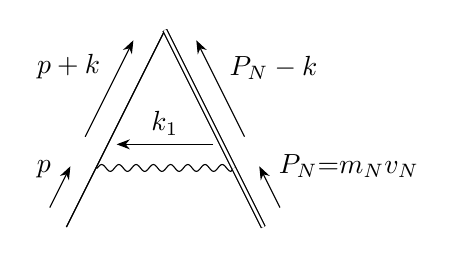
\begin{tikzpicture}[baseline=($(p1)!0.5!(x)$)]
	\begin{feynman}
    \vertex (p1);
	\vertex[right=2.5cm of p1] (p2);
	\vertex at ($(p1)!0.5!(p2)+(0,2.5cm)$) (x) ;
	\vertex at ($(p1)!0.3!(x)$) (y1);
	\vertex at ($(p2)!0.3!(x)$) (z1);
	%
	\diagram* {
	  (p1) -- [] (x);
	  (p2) -- [double distance=1pt] (x);
	  (y1) -- [photon,rmomentum=$k_1$] (z1);
	  (p1) -- [momentum=\(p\)] (y1);
	  (p2) -- [momentum'=$P_{N}\text{=}m_{N}v_{N}$,double distance=1pt] (z1);
	  (y1) -- [momentum=\(p+k\)] (x);
	  (z1) -- [momentum'=\(P_{N}-k\),double distance=1pt] (x);
    };
	\end{feynman}
  \end{tikzpicture}
\end{align*}
which doesn't have logarithm divergence\footnote{After dimensional regularization, the Gamma function in the numerator is something like $\Gamma(n-d/2)$ and Gamma function doesn't have pole at half integer. }. 
\subsection{NNLO}
\begin{align*}
  &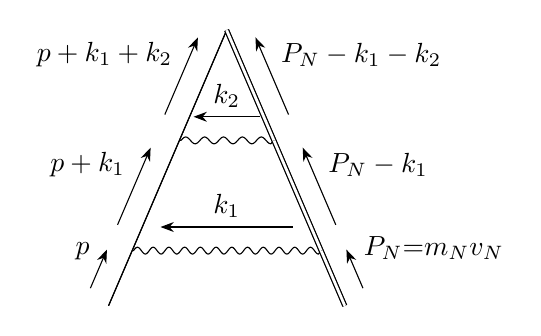
\begin{tikzpicture}[baseline=($(p1)!0.5!(x)$)]
 \begin{feynman}
   \vertex (p1);
 \vertex[right=3cm of p1] (p2);
 \vertex at ($(p1)!0.5!(p2)+(0,3.5cm)$) (x) ;
 \vertex at ($(p1)!0.2!(x)$) (y1);
 \vertex at ($(p2)!0.2!(x)$) (z1);
 \vertex at ($(p1)!0.6!(x)$) (y2);
 \vertex at ($(p2)!0.6!(x)$) (z2);
 %
 \diagram* {
   (p1) -- [] (x);
   (p2) -- [double distance=1pt] (x);
   (y1) -- [photon,rmomentum=$k_1$] (z1);
   (y2) -- [photon,rmomentum=$k_2$] (z2);
   (p1) -- [momentum=\(p\)] (y1);
   (p2) -- [momentum'=$P_{N}\text{=}m_{N}v_{N}$,double distance=1pt] (z1);
   (y1) -- [momentum=\(p+k_1\)] (y2);
   (z1) -- [momentum'=\(P_{N}-k_1\),double distance=1pt] (z2);
   (y2) -- [momentum=\(p+k_1+k_2\)] (x);
   (z2) -- [momentum'=\(P_{N}-k_1-k_2\),double distance=1pt] (x);
   };
 \end{feynman}
 \end{tikzpicture}\\ =&-\mu^{-4\epsilon}e^4\bqty{\int[dk_1][dk_2]\frac{1}{\vb{\abs{k_1}}^2}\frac{1}{\vb{\abs{k_2}}^2}\frac{1}{-k_1^0-k_2^0+i\epsilon}\frac{1}{-k_1^0+i\epsilon}\frac{2m+2E+k_1^0}{p^0+k_1^0-m-\frac{\vb{(p+k_1)}^2}{2m}+i\epsilon}\frac{2m+2E+2k_1^0+k_2^0}{p^0+k_1^0+k_2^0-m-\frac{\vb{(p+k_1+k_2)}^2}{2m}+i\epsilon}}
 \\
 \intertext{do the shift as above}
 =&e^4\bqty{\int\frac{\dd^3\vb{k_1}}{(2\pi)^3}\frac{\dd^3\vb{k_2}}{(2\pi)^3}\frac{1}{\vb{\abs{k_1-p}}^2}\frac{1}{\vb{\abs{k_2-k_1}}^2}\frac{2m+2E}{E-\frac{\vb{\abs{k_1}}^2}{2m}+2i\epsilon}\frac{2m+2E}{E-\frac{\vb{\abs{k_2}}^2}{2m}+2i\epsilon}}\\
\end{align*}
\begin{align*}
  &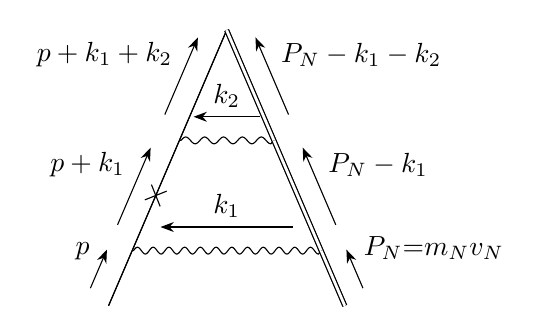
\begin{tikzpicture}[baseline=($(p1)!0.5!(x)$)]
 \begin{feynman}
   \vertex (p1);
 \vertex[right=3cm of p1] (p2);
 \vertex at ($(p1)!0.5!(p2)+(0,3.5cm)$) (x) ;
 \vertex at ($(p1)!0.2!(x)$) (y1);
 \vertex at ($(p2)!0.2!(x)$) (z1);
 \vertex at ($(p1)!0.6!(x)$) (y2);
 \vertex at ($(p2)!0.6!(x)$) (z2);
 \vertex at ($(y1)!0.5!(z1)$) (t);
 %
 \diagram* {
   (p1) -- [] (x);
   (p2) -- [double distance=1pt] (x);
   (y1) -- [photon,rmomentum=$k_1$] (z1);
   (y2) -- [photon,rmomentum=$k_2$] (z2);
   (p1) -- [momentum=\(p\)] (y1);
   (p2) -- [momentum'=$P_{N}\text{=}m_{N}v_{N}$,double distance=1pt] (z1);
   (y1) -- [momentum=\(p+k_1\),insertion=0.5] (y2);
   (z1) -- [momentum'=\(P_{N}-k_1\),double distance=1pt] (z2);
   (y2) -- [momentum=\(p+k_1+k_2\)] (x);
   (z2) -- [momentum'=\(P_{N}-k_1-k_2\),double distance=1pt] (x);
   };
 \end{feynman}
 \end{tikzpicture}=16m^2(m+E)\mu^{-4\epsilon}e^4
 \int\frac{\dd^3\vb{k_1}}{(2\pi)^3}\frac{\dd^3\vb{k_2}}{(2\pi)^3}\frac{1}{\vb{\abs{k_1-p}}^2}\frac{1}{\vb{\abs{k_2-k_1}}^2}\frac{\vb{\abs{k_1}}^4/4m^2}{[\vb{\abs{k_1}}^2-2mE]^2}\frac{1}{\vb{\abs{k_2}}^2-2mE}\\
  =&16m^2(m+E)\mu^{-4\epsilon}e^4\int_0^1\dd x\int\frac{\dd^3\vb{k_1}}{(2\pi)^3}\frac{1}{\vb{\abs{k_1-p}}^2}\frac{\vb{\abs{k_1}}^4/4m^2}{[\vb{\abs{k_1}}^2-2mE]^2}\frac{\left(\frac{4 \pi }{\Delta_2 }\right)^{2-\frac{d}{2}} \Gamma \left(2-\frac{d}{2}\right)}{(4 \pi )^2 \Gamma (2)}\\
  \intertext{where $\Delta_2=(1-x) \left(\vb{\abs{k_1}}^2 x-2 E m\right)$} 
  =&16m^2(m+E)\mu^{-4\epsilon}e^4\frac{1}{(4\pi)^2}\int_0^1\dd x\int\frac{\dd^3\vb{k_1}}{(2\pi)^3}\frac{1}{\vb{\abs{k_1-p}}^2}\frac{\vb{\abs{k_1}}^4/4m^2}{[\vb{\abs{k_1}}^2-2mE]^2}\frac{1}{(\vb{\abs{k_1}}^2-2mE/x)^{2-d/2}}\pqty{\frac{4\pi}{x(1-x)}}^{2-d/2}\Gamma(2-d/2)\\
  =&16m^2(m+E)\mu^{-4\epsilon}e^4\frac{1}{(4\pi)^2}\int_0^1\dd x\int_0^1\dd y\dd z\dd t\delta(y+z+t-1)\int\frac{\dd^3 \vb{k_1}}{(2\pi)^3}\frac{zt^{1-d/2}\vb{\abs{k_1}}^4/4m^2}{[\vb{\abs{k_1}}^2+\Delta_1]^{5-d/2}}\frac{\Gamma(5-d/2)}{\Gamma(2-d/2)}\pqty{\frac{4\pi}{x(1-x)}}^{2-d/2}\Gamma(2-d/2)\\
  \intertext{where $\Delta_1=y(1-y)\vb{p}^2-2mE(z+t/x)$}
  =&16m^2(m+E)\mu^{-4\epsilon}e^4\frac{1}{4m^2(4\pi)^2}\int_0^1\dd x\int_0^1\dd y\dd z\dd t\delta(y+z+t-1)zt^{1-d/2}\frac{d (d+2)}{4}\frac{\Gamma \left(3-d\right)}{(4 \pi )^{3-d/2} } \left(\frac{4 \pi }{\Delta_1 }\right)^{3-d} \pqty{\frac{4\pi}{x(1-x)}}^{2-d/2}\\
  =&-16m^2(m+E)\frac{1}{128 \pi ^2  m^2}(\frac{1}{d-3}+4 \log{\mu})+\text{finite terms}
\end{align*}
\begin{align*}
  &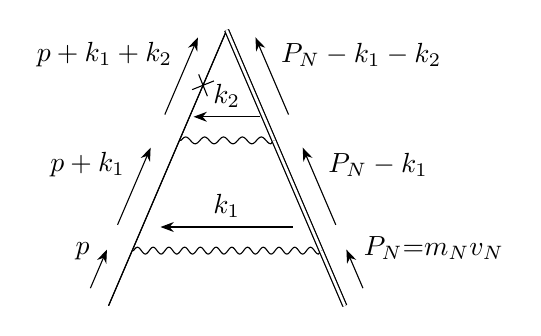
\begin{tikzpicture}[baseline=($(p1)!0.5!(x)$)]
 \begin{feynman}
   \vertex (p1);
 \vertex[right=3cm of p1] (p2);
 \vertex at ($(p1)!0.5!(p2)+(0,3.5cm)$) (x) ;
 \vertex at ($(p1)!0.2!(x)$) (y1);
 \vertex at ($(p2)!0.2!(x)$) (z1);
 \vertex at ($(p1)!0.6!(x)$) (y2);
 \vertex at ($(p2)!0.6!(x)$) (z2);
 \vertex at ($(y1)!0.5!(z1)$) (t);
 %
 \diagram* {
   (p1) -- [] (x);
   (p2) -- [double distance=1pt] (x);
   (y1) -- [photon,rmomentum=$k_1$] (z1);
   (y2) -- [photon,rmomentum=$k_2$] (z2);
   (p1) -- [momentum=\(p\)] (y1);
   (p2) -- [momentum'=$P_{N}\text{=}m_{N}v_{N}$,double distance=1pt] (z1);
   (y1) -- [momentum=\(p+k_1\)] (y2);
   (z1) -- [momentum'=\(P_{N}-k_1\),double distance=1pt] (z2);
   (y2) -- [momentum=\(p+k_1+k_2\),insertion=0.5] (x);
   (z2) -- [momentum'=\(P_{N}-k_1-k_2\),double distance=1pt] (x);
   };
 \end{feynman}
 \end{tikzpicture}=16m^2(m+E)
   \mu^{-4\epsilon}e^4\int\frac{\dd^3\vb{k_1}}{(2\pi)^3}\frac{\dd^3\vb{k_2}}{(2\pi)^3}\frac{1}{\vb{\abs{k_1-p}}^2}\frac{1}{\vb{\abs{k_2-k_1}}^2}\frac{1}{\vb{\abs{k_1}}^2-2mE}\frac{\vb{\abs{k_2}}^4/4m^2}{[\vb{\abs{k_2}}^2-2mE]^2}\\
  =&16m^2(m+E)\mu^{-4\epsilon}e^4\frac{1}{4m^2}\int_0^1\dd x\int\frac{\dd^3\vb{k_1}}{(2\pi)^3}\frac{1}{\abs{\vb{k_1-p}}^2}\frac{1}{\vb{\abs{k_1}}^2-2mE}\frac{(1-x)\Gamma(1-d/2)}{8\pi}\pqty{\frac{4\pi}{\Delta_2}}^{1-d/2}\frac{d(d+2)}{4}\\
  \intertext{where $\Delta_2=x(1-x)\vb{\abs{k_1}}^2-2mE(1-x)$}
  =&16m^2(m+E)\mu^{-4\epsilon}e^4\frac{1}{4m^2}\int_0^1\dd x\int_0^1\dd y\dd z\dd t\frac{t^{-d/2}}{[\vb{\abs{k_1}}^2+\Delta_1]^{3-d/2}}\frac{\Gamma{(3-d/2)}}{\Gamma{(1-d/2)}}\delta(y+z+t-1)\frac{\Gamma(1-d/2)}{8\pi}\pqty{\frac{4\pi}{x(1-x)}}^{1-d/2}\frac{d(d+2)x}{4}\\
  \intertext{where $\Delta_1=y(1-y)\vb{p}^2-2mEz-2mE\frac{t}{x }$}
  =&16m^2(m+E)\mu^{-4\epsilon}e^4\frac{1}{4m^2}\int_0^1\dd x\int_0^1\dd y\dd z\dd t\delta(y+z+t-1)\frac{1}{(4\pi)^{3-d/2}} \left(\frac{4 \pi }{\Delta_1 }\right)^{3-d} \frac{\Gamma \left(3-d\right)}{8\pi}\pqty{\frac{4\pi}{x(1-x)}}^{1-d/2}\frac{d(d+2)x}{4}t^{-d/2}\\
  =&16m^2(m+E)\frac{15}{8192 \pi ^2  m^2}(\frac{1}{d-3}+4 \log{\mu})+\text{finite terms}
\end{align*}

\clearpage
\begin{appendices}
  Integral with the structure of the form 
  \begin{align*}
	\int[dk_1][dk_2]\frac{1}{\vb{\abs{k_1}}^2}\frac{1}{\vb{\abs{k_2}}^2}\frac{1}{-k_1^0-k_2^0+i\epsilon}\frac{1}{-k_1^0+i\epsilon}\frac{1}{[p^0+k_1^0-m-\frac{\vb{(p+k_1)}^2}{2m}+i\epsilon]^m}\frac{1}{[p^0+k_1^0+k_2^0-m-\frac{\vb{(p+k_1+k_2)}^2}{2m}+i\epsilon]^n}
  \end{align*}
  will always produce
  \begin{align*}
	\int\frac{\dd^3\vb{k_1}}{(2\pi)^3}\frac{\dd^3\vb{k_2}}{(2\pi)^3}\frac{1}{\vb{\abs{k_1}}^2}\frac{1}{\vb{\abs{k_2}}^2}\frac{1}{[p^0-m-\frac{\vb{(p+k_1)}^2}{2m}]^m}\frac{1}{[p^0-m-\frac{\vb{(p+k_1+k_2)}^2}{2m}+i\epsilon]^n}
  \end{align*}
  with $k_1^0$ and $k_2^0$ goes to zero.

  For arbitary one loop diagram of the following form, we have
  \begin{subequations} \label{1loopgamma}
	\begin{align}
	  \int\frac{\dd^dk}{(2\pi)^d}\frac{k^{2\b}}{(k^2+\Delta)^n}&=\frac{1}{(4\pi)^{n-\b}}\frac{\Gamma(\b+d/2)}{\Gamma(d/2)}\frac{\Gamma(n-\b-d/2)}{\Gamma(n)}\pqty{\frac{4\pi}{\Delta}}^{n-\b-d/2}\\
	  &=\frac{1}{(4\pi)^{d/2}}\frac{\Gamma(\b+d/2)}{\Gamma(d/2)}\frac{\Gamma(n-\b-d/2)}{\Gamma(n)}\pqty{\frac{1}{\Delta}}^{n-\b-d/2}
	\end{align}
  \end{subequations}
  For two loop diagrams of this form ($\epsilon=3-d$)
  \begin{align}
	\mu^{-4\epsilon}\int\frac{\dd^d\vb{k}_1}{(2\pi)^d}\frac{\dd^d\vb{k}_2}{(2\pi)^d}\frac{1}{\vb{(k_1-a)}^2}\frac{1}{\vb{(k_2-k_1)}^2}\frac{\vbk_1^{2\a}}{(\vb{k}_1^2-c)^m}\frac{\vbk_2^{2\b}}{(\vb{k}_2^2-d)^n}
	\label{int}
  \end{align}
  The integral is evaluated to
  \begin{align*}
	&\mu^{-4\epsilon}\int_0^1\prod_{i=1}^2\dd x_i\delta(\sum x_i-1)\prod x_i^{d_i-1}\frac{\Gamma(n+1)}{\Gamma(n)}\frac{1}{(4\pi)^{n+1-\b}}\frac{\Gamma(\b+d/2)}{\Gamma(d/2)}\frac{\Gamma(n+1-\b-d/2)}{\Gamma(n+1)}\pqty{\frac{4\pi}{\a(x_i)}}^{n+1-\b-d/2}
	\\&\int\frac{\dd^d\vb{k}_1}{(2\pi)^d}\frac{1}{\vb{(k_1-a)}^2}\frac{\vbk_1^{2\a}}{(\vb{k}_1^2-c)^m}\frac{1}{(\vb{k}_1-\Delta_2)^{n+1-\b-d/2}}\\
	=&\mu^{-4\epsilon}\int_0^1\prod_{i=1}^2\dd x_i\delta(\sum x_i-1)\prod x_i^{d_i-1}\frac{1}{(4\pi)^{n+1-\b}}\frac{\Gamma(\b+d/2)}{\Gamma(d/2)}\frac{\Gamma(n+1-\b-d/2)}{\Gamma(n)}\pqty{\frac{4\pi}{\a(x_i)}}^{n+1-\b-d/2}\int_0^1\prod_{i=1}^3\dd y_j\delta(\sum y_j-1)\prod y_j^{d_j-1}
	\\&\frac{\Gamma(m+n+2-\b-d/2)}{\Gamma(m)\Gamma(n+1-\b-d/2)}\frac{1}{(4\pi)^{m+n+2-\a-\b-d/2}}\frac{\Gamma(\a+d/2)}{\Gamma(d/2)}\frac{\Gamma(m+n+2-\a-\b-d)}{\Gamma(m+n+2-\b-d/2)}\pqty{\frac{4\pi}{\Delta_1}}^{m+n+2-\a-\b-d}
	\\
	=&\mu^{-4\epsilon}\int_0^1\prod_{i=1}^2\dd x_i\delta(\sum x_i-1)\prod x_i^{d_i-1}\frac{1}{(4\pi)^{d}}\frac{\Gamma(\b+d/2)}{\Gamma(d/2)}\frac{1}{\Gamma(n)}\pqty{\frac{1}{\a(x_i)}}^{n+1-\b-d/2}
	\\&\int_0^1\prod_{i=1}^3\dd y_j\delta(\sum y_j-1)\prod y_j^{d_j-1}\frac{\Gamma(\a+d/2)}{\Gamma(d/2)}\frac{\Gamma(m+n+2-\a-\b-d)}{\Gamma(m)}\pqty{\frac{1}{\Delta_1}}^{m+n+2-\a-\b-d}
  \end{align*}<++>
\end{appendices}

\end{document}
